\subsection{Coherency score}
\frame
{
	\frametitle{Coherency score calculation}
		
	\begin{columns}[T]
	\column{.5\textwidth}
	\begin{itemize}
		\small
		\item Coherency over temporal window 
		\item Parameters:
			\begin{itemize}
				\item $\tau_w$ - window size
				\item \# appearing nodes
				\item \# disappearing nodes
				\item node weights - $\rho^l_i$
			\end{itemize}
		\begin{figure}[p]
			\centering
			\hspace{-1cm}
			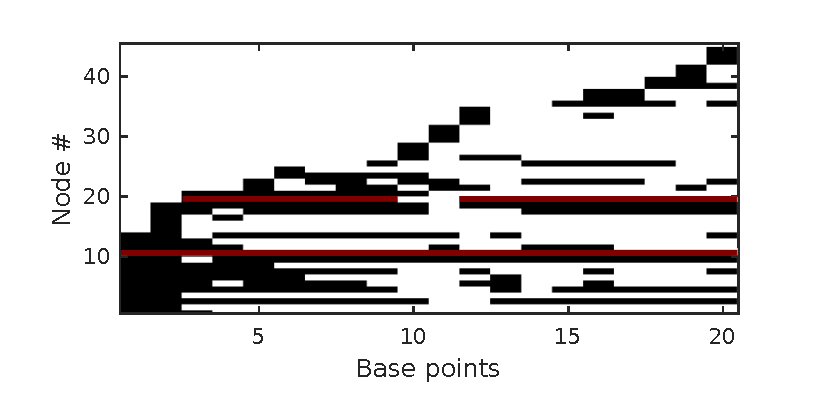
\includegraphics[width = 1\textwidth]{img/icsc/node_continuity.eps}
			\label{fig:coh_score_3}
		\end{figure}
	\end{itemize}
	\column{.6\textwidth}
	\hspace{-2cm}
	\small
	\begin{align}
	\varphi^k &= 1 - \sum\limits_{l=k-\tau_w}^{k}\sum\limits_{i=1}^{\lvert n^l \rvert}\rho^{l}_i (a^{l}_i + b^{l}_i) \label{eq:incoherency_score}	\end{align}
	where
	\begin{align}
	a^l_i &= \begin{cases}
	1 &\text{if }	M_{li}>0, \, M_{l-1,i}=0 \\
	0 &\text{otherwise}
	\end{cases}  \label{eq:a}	\\
	b^l_i &= \begin{cases}
	1 &\text{if }	M_{li}=0,  M_{l-1,i}>0 \\
	0 &\text{otherwise}
	\end{cases}  \label{eq:b}	\\
	\rho^l_i &\propto s_3(N^l_i) 
	\times \sum\limits_{k=l-{\tau_w}}^{l} M_{ki}>0 \label{eq:rho}									
	\end{align}

	\end{columns}
}
\subsection{Place Detection}
\frame
{
	\frametitle{Place Detection}
	
	\begin{columns}[t,onlytextwidth]
		\hspace*{-1cm}
		
		\column{.99\textwidth}
		\vspace{-0.5cm}
		\begin{figure}[p]
			\centering
			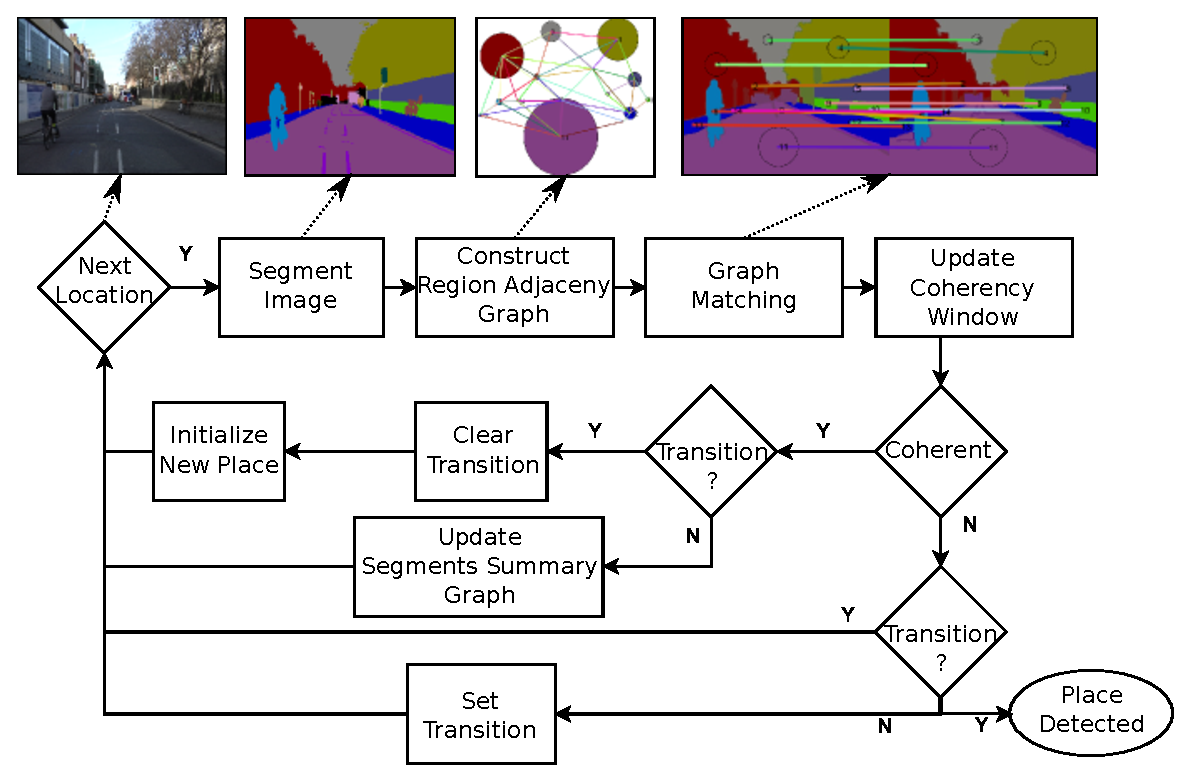
\includegraphics[width = 0.9\textwidth]{img/icsc/diagram}
		\end{figure}
		
	\end{columns}
}